\chapter{LDA of Investments in the United States} 
\section{Introduction}
\nocite{tmpackage} \nocite{LDAvis} \nocite{Stargazer}
\nomenclature{MPT}{Modern Portfolio Theory}	

While Chapter \ref{chapterIV} explored the locational preferences of institutional investors in the US as a whole and in the five largest American metropolitan areas by total funds under management, this chapter will explore whether geography can play a role in individual investors portfolio choices.   

While Modern Portfolio Theory (MPT), as established by \cite{Markowitz1952} advocates for holding a broad and negatively correlated portfolio, the notion of "not putting all of one's eggs in a single basket" is an old one, for \cite{Lofthouse53} finds that such advice was formally practised by the British investment firm Investment Registry as far back as 1904.  

In concert with MPT's emphasis on diversification, the reaction to the Crash of October 1987 placed renewed emphasis on risk management and the rise of ``Value at Risk'' (VAR) based investing in which firms would try to maximise returns while minimizing risk.  This led to a homogenizing effect in investment strategies as explained by Andrew G. Haldane executive director of Financial Stability at the Bank of England at a conference on risk management:

\nomenclature{VAR}{Value at Risk}
\begin{quote}
	Within the financial sector, diversity appears to have been reduced for two separate, but related, reasons:  the pursuit of return;  and the management of risk.  The pursuit of yield resulted in a return on equity race among all types of financial firm.  As they collectively migrated to high-yield activities, business strategies came to be replicated across the financial sector.  Imitation became the sincerest form of flattery.
	
	So savings cooperatives transformed themselves into private commercial banks.  Commercial banks ventured into investment banking.  Investment banks developed in-house hedge funds through large proprietary trading desks.  Funds of hedge funds competed with traditional investment funds.  And investment funds - pension, money market mutual, insurance - imported the risk the others were shedding.   \citep[p.18]{Haldane2009}
\end{quote} 

As explored in Chapter \ref{ChapterII}, there is a substantial literature showing that stock pickers are biased towards industries in which they are knowledgeable or have personal connections.  In particular, \cite{covalthe2001} find that investors can draw abnormally high returns from local knowledge, and another study by \cite{Cohen2008} makes a compelling case that stock pickers are biased towards selecting stocks of companies that their board of directors contain shared alumni networks.  

Rather than looking at geographic differences of investors based on the type of institution they belong to such as but not limited to banks, hedge funds, pension funds, and insurance companies, this study will attempt to create functional portfolio archetypes using machine learning and aggregate these archetypes by geography in order to look for regional patterns.   

\section{Latent Dirichlet allocation}

\nomenclature{LDA}{Latent Dirichlet allocation}

Latent Dirichlet allocation (LDA) \nomenclature{LDA}{Latent Dirichlet allocation} is a generative statistical technique developed by David Blei to find themes that are common across a corpus of texts \citep{blei2003latent}.  This technique is a derivation and refinement of \cite{Papadimitriou98} and \cite{PAPADIMITRIOU2000217} work on Latent Semantic Indexing.  

LDA has made certain classification tasks feasible to conduct in a short time, such as analysing a large sample of digitized 18th century American newspapers for the topics of the day that would otherwise be unfeasible for any individual to read \citep{newman2006probabilistic}.  Another well known use of LDA is for finding in near-realtime the topics of controversy and/or debate at an academic conference via Twitter usage by the participants of the conference \citep{Marwick2013}.

In addition to text analysis, LDA has been used in multiple different fields such as finding latent patterns in biodiversity data \citep{Vale2014}, genetic data, images, social networks \citep{Blei2012} as well as remote sensing data \citep{Lienou2010}.

\subsection{How does LDA work?}

Ted Underwood, who studies the intersection of Information Science and English Literature, contends in his academic blog post entitled ``Topic modeling made just simple enough[sic]" that academic papers make LDA look much harder than it is in practice, since their main goal is to show how and why their underlying formulas work and the mathematical proofs rely on highly advanced mathematics. If we take the algorithms to work as intended, the practice of LDA can be easily explained in practice \citep{Underwood2012}.

LDA assumes that each document being analyzed contains a multitude of different topics, and each of these topics are latent, that is to say they can't be directly observed, but can be defined indirectly. Edwin Chen's classic introduction to LDA example is quite straight forward \citep{Chen2011}.  Take the following five sentences:

\begin{enumerate}
	\singlespacing 
	\item I like to eat broccoli and bananas.
	\item I ate a banana and spinach smoothie for breakfast.
	\item Chinchillas and kittens are cute.
	\item My sister adopted a kitten yesterday.
	\item Look at this cute hamster munching on a piece of broccoli.
\end{enumerate}

If we treat each sentence as a document for LDA purposes, and we were to limit ourselves to two topics, we would see something to the effect of the following:

\begin{itemize}
	\item \textbf{Sentences 1 and 2:} 100\% topic A
	\item \textbf{Sentences 3 and 4:} 100\% topic B
	\item \textbf{Sentence 5:} 60\% topic A, 40\% topic B
\end{itemize}

At this point, we see that the topics consists of:
\begin{itemize}	
	\item \textbf{topic A:} 30\% broccoli, 15\% bananas, 10\% breakfast, 10\% munching, etc... 
	
	\item \textbf{topic B:} 20\% chinchillas, 20\% kittens, 20\% cute, 15\% hamster, etc...  
\end{itemize}

At which point, we can see that topic A consists mostly of food and food adjacent activities, whereas topic B is about animals and their general cuteness. 

At this point, it is important to state that LDA assumes that language is a "bag of words". That is to say that for the purpose of the model, the order of words and punctuation isn't considered important information.  While this may cause some miss-coding of information in a limited context, since grammar, punctuation and word order can relay important information, larger corpora smooth-out these ambiguities. For example, an LDA model would treat the following two sentences as being identical:

\begin{itemize}	
	\item  Have you eaten, my child?
	
	\item  Have you eaten my child\textinterrobang 
\end{itemize}

This study will be using LDA on Stock unique identifiers (CUSIP). The "bag of words" methodology works to our advantage since the presented order of stocks in an institutional investor's portfolio will not influence the sorting algorithm. Relative location agnosticism is useful in this case since unlike earth movers' distance classification \citep{rubner2000earth} this method of classification isn't dependant on the initial relative distribution within the input variables, and therefore there is no need for a special ordering of stock positions in the input file.  


The LDA process is mapped out graphically in Figure \ref{fig:LDA_graphic} and written out in Equation \ref{LDAequation}. 


\begin{equation}
P(Z|W,D) = \dfrac{\# \text{ of words } W \text{ in topic } Z + \beta_{w}}{\text{total tokens in } Z + \beta}*(\# \text{ of words in } D \text{ that belong to } Z + \alpha)
\label{LDAequation}
\end{equation}



\begin{figure}[H]
	\tikzset{every picture/.style={line width=0.75pt}} %set default line width to 0.75pt        
	
	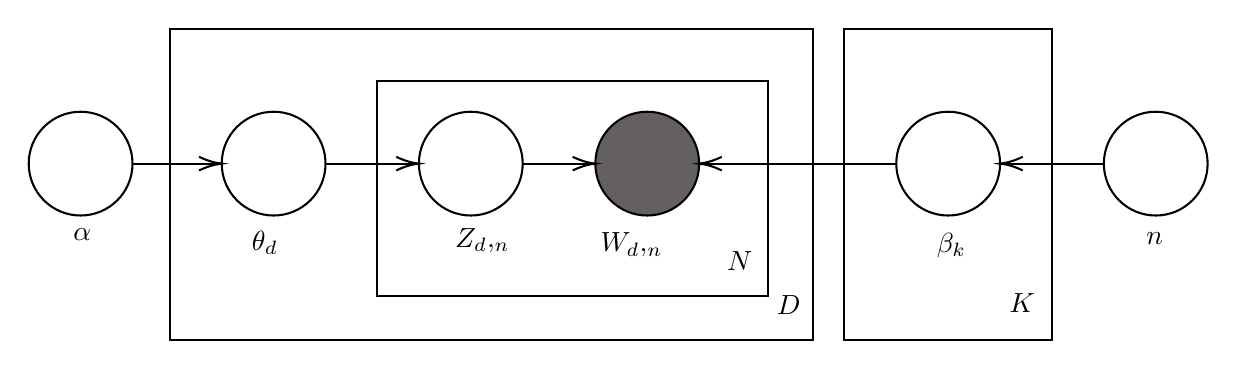
\begin{tikzpicture}[x=0.75pt,y=0.75pt,yscale=-1,xscale=1]
	%uncomment if require: \path (0,179); %set diagram left start at 0, and has height of 179
	
	%Shape: Rectangle [id:dp21726410884148195] 
	\draw   (235,38) -- (423,38) -- (423,142) -- (235,142) -- cycle ;
	%Shape: Rectangle [id:dp8470156804479287] 
	\draw   (135,13) -- (445,13) -- (445,163) -- (135,163) -- cycle ;
	%Shape: Rectangle [id:dp5437180445728402] 
	\draw   (460,13) -- (560,13) -- (560,163) -- (460,163) -- cycle ;
	%Shape: Circle [id:dp6027361372166333] 
	\draw   (67,78) .. controls (67,64.19) and (78.19,53) .. (92,53) .. controls (105.81,53) and (117,64.19) .. (117,78) .. controls (117,91.81) and (105.81,103) .. (92,103) .. controls (78.19,103) and (67,91.81) .. (67,78) -- cycle ;
	%Shape: Circle [id:dp5441473658198903] 
	\draw   (160,78) .. controls (160,64.19) and (171.19,53) .. (185,53) .. controls (198.81,53) and (210,64.19) .. (210,78) .. controls (210,91.81) and (198.81,103) .. (185,103) .. controls (171.19,103) and (160,91.81) .. (160,78) -- cycle ;
	%Shape: Circle [id:dp028671426160656655] 
	\draw   (255,78) .. controls (255,64.19) and (266.19,53) .. (280,53) .. controls (293.81,53) and (305,64.19) .. (305,78) .. controls (305,91.81) and (293.81,103) .. (280,103) .. controls (266.19,103) and (255,91.81) .. (255,78) -- cycle ;
	%Shape: Circle [id:dp6901716019104538] 
	\draw  [fill={rgb, 255:red, 101; green, 96; blue, 96 }  ,fill opacity=1 ] (340,78) .. controls (340,64.19) and (351.19,53) .. (365,53) .. controls (378.81,53) and (390,64.19) .. (390,78) .. controls (390,91.81) and (378.81,103) .. (365,103) .. controls (351.19,103) and (340,91.81) .. (340,78) -- cycle ;
	%Shape: Circle [id:dp7815059339533368] 
	\draw   (485,78) .. controls (485,64.19) and (496.19,53) .. (510,53) .. controls (523.81,53) and (535,64.19) .. (535,78) .. controls (535,91.81) and (523.81,103) .. (510,103) .. controls (496.19,103) and (485,91.81) .. (485,78) -- cycle ;
	%Shape: Circle [id:dp45137687393472814] 
	\draw   (585,78) .. controls (585,64.19) and (596.19,53) .. (610,53) .. controls (623.81,53) and (635,64.19) .. (635,78) .. controls (635,91.81) and (623.81,103) .. (610,103) .. controls (596.19,103) and (585,91.81) .. (585,78) -- cycle ;
	%Straight Lines [id:da3313227430829817] 
	\draw    (117,78) -- (158,78) ;
	\draw [shift={(160,78)}, rotate = 180] [color={rgb, 255:red, 0; green, 0; blue, 0 }  ][line width=0.75]    (10.93,-3.29) .. controls (6.95,-1.4) and (3.31,-0.3) .. (0,0) .. controls (3.31,0.3) and (6.95,1.4) .. (10.93,3.29)   ;
	%Straight Lines [id:da2686493807462953] 
	\draw    (210,78) -- (253,78) ;
	\draw [shift={(255,78)}, rotate = 180] [color={rgb, 255:red, 0; green, 0; blue, 0 }  ][line width=0.75]    (10.93,-3.29) .. controls (6.95,-1.4) and (3.31,-0.3) .. (0,0) .. controls (3.31,0.3) and (6.95,1.4) .. (10.93,3.29)   ;
	%Straight Lines [id:da5780607817492671] 
	\draw    (305,78) -- (338,78) ;
	\draw [shift={(340,78)}, rotate = 180] [color={rgb, 255:red, 0; green, 0; blue, 0 }  ][line width=0.75]    (10.93,-3.29) .. controls (6.95,-1.4) and (3.31,-0.3) .. (0,0) .. controls (3.31,0.3) and (6.95,1.4) .. (10.93,3.29)   ;
	%Straight Lines [id:da026847412265174286] 
	\draw    (485,78) -- (392,78) ;
	\draw [shift={(390,78)}, rotate = 360] [color={rgb, 255:red, 0; green, 0; blue, 0 }  ][line width=0.75]    (10.93,-3.29) .. controls (6.95,-1.4) and (3.31,-0.3) .. (0,0) .. controls (3.31,0.3) and (6.95,1.4) .. (10.93,3.29)   ;
	%Straight Lines [id:da15128656608765012] 
	\draw    (585,78) -- (537,78) ;
	\draw [shift={(535,78)}, rotate = 360] [color={rgb, 255:red, 0; green, 0; blue, 0 }  ][line width=0.75]    (10.93,-3.29) .. controls (6.95,-1.4) and (3.31,-0.3) .. (0,0) .. controls (3.31,0.3) and (6.95,1.4) .. (10.93,3.29)   ;
	
	% Text Node
	\draw (87,107.9) node [anchor=north west][inner sep=0.75pt]    {$\alpha $};
	% Text Node
	\draw (173,108.9) node [anchor=north west][inner sep=0.75pt]    {$\theta _{d}$};
	% Text Node
	\draw (271,107.9) node [anchor=north west][inner sep=0.75pt]    {$Z_{d} ,_{n}$};
	% Text Node
	\draw (402,118.9) node [anchor=north west][inner sep=0.75pt]    {$N$};
	% Text Node
	\draw (341,109.9) node [anchor=north west][inner sep=0.75pt]    {$W_{d},_{n}$};
	% Text Node
	\draw (426,139.9) node [anchor=north west][inner sep=0.75pt]    {$D$};
	% Text Node
	\draw (503,109.9) node [anchor=north west][inner sep=0.75pt]    {$ \beta_{k}$};
	% Text Node
	\draw (538,138.9) node [anchor=north west][inner sep=0.75pt]    {$K$};
	% Text Node
	\draw (604,109.9) node [anchor=north west][inner sep=0.75pt]    {$n$};
	
	
	\end{tikzpicture}
	\caption[Graphical Model of Latent Dirichlet allocation]{Graphical model of Latent Dirichlet allocation replicated from the graphic in Blei (2012), where K is the total number of topics, $ \beta _{k}$ is the topic, a distribution over the vocabulary, $D$ is the total number of documents, $\Theta_{d}$ is the per-document topic proportions, N is the total number of words in a document, $Z_{d},_{n}$ is the per-word topic assignment, $W_{d},_{n}$ observed word, and finally $\alpha$ and $n$ as dirichlet parameters. }
	
	\label{fig:LDA_graphic}
\end{figure}



\section{Preparing the Data}
A closer analogue to using LDA is using this technique to classifying card selection in games such as Magic: The Gathering \citep{Hlynsson2017}.  This collectible card game uses 60 cards decks that are selected ahead of time by the player.  Due to the game's complex resource system and multiple different strategies for attacking one's opponent, cards are not fungible, and thus the game consolidates towards certain discreet collection of cards.  Similarly, the use LDA can be used to aggregate different stock portfolios into different investment strategies.  

In order to conduct an LDA analysis, the data was taken from the XBRL database of 13-F HR database for the period of the second quarter of 2013 to the end of 2018.  The process used in collecting and cleaning this data was explained in Chapter \ref{Section:13F}.  

Unfortunately the database had to be pruned of all holdings of less than 1 million dollars so that the matrix operations conducted by the LDA package would fit within the computer's available RAM (Random Access Memory)\footnote{At the time, these computers contained 32gb of RAM.}.   This value of 1 million dollars was achieved in an iterative manner, with one computer starting with all transactions above 10 million dollars and reducing this threshold by 1 million USD every time the LDA converged on a solution and a second computer starting with all transactions and pruning by increments of 100 000 USD until the algorithm converged rather than crash the program due to overwhelming the available RAM.  Furthermore, due to the nature of the LDA algorithm (needing full matrix operations), it was unfeasible to spread the workload across multiple computers, nor to slice the program into year-long slices and perform 5 LDA analyses, since this would give us the worst of both worlds - no time continuity and the multiple testing problem. 

In practice, this reduces the size of the database from 92 702 to 91 270 filers/quarters.  That being said, the pruning of the database focuses the analysis on stock positions that have substantial, if theoretical, corporate power\footnote{Such as but not limited to voting rights and the threat of lowering stock prices in a mass sell-off being the best alternative to a negotiated solution.} rather than holdings that are simply intended passively to accrue in value and render dividends as part of a diversification strategy under the modern portfolio theory.

Furthermore, in this LDA analysis each filer-quarter is treated as independent filers in the LDA model. Stock positions do shift over time to the point that acting on information 45 days old can be ruinous, a fact that many whale watchers repeat in their newsletters and news reports \citep{Whale_Watching_CNBC_12,cramerwhale}. Since stock positions shift over time to newer strategies, this should not pose a problem; for example this would treat a caterpillar and a butterfly differently.  While indubitably the same creature, the caterpillar and the butterfly look, act, and occupy different ecological niches.  This returns to the lumper-splitter problem. In this case, do we value tracing the metamorphosis or the different niches both ends occupy?  This treatment of investors and filing periods as discrete periods allows for the tracing of an investor's strategy shifting from predominantly X to predominantly Y.  However, since the follow-on analysis will take time into effect, not having it in the original training model is simply a nod to feasibility. 

Literary-based LDA suggests removing stop words.  These words comprise grammatical objects such as but not limited to pronouns, common adjectives and articles that make text understandable, but don't necessarily convey the latent topic. For example, any LDA analysis that uses English language prose would be overwhelmed by articles such as "the". The inclusion of such a word would saturate any analysis of Sherlock Holmes books by Arthur Conan Doyle \citep{Silge2018}.  That being said, there are no "words" - that is to say stock CUISP - that are as common as the word "the" in this analysis.  In fact the most common CUSIP in the training database is CUSIP 037833100 (Apple Inc.) accounting for approximately one percent of all positions in the pruned database. While this popularity should not be surprising considering Apple's status in the investing world during the late aughts and the early to mid twenty-tens, this is nowhere as common as "the" or "they" in English prose.   

Another practice that is common in literary-based uses of LDA is stemming words. This removes prefixes and suffixes of words such that only their roots are used.  For example, faster and fastest relate the same idea -- fast.  However, since the words used in this analysis are in-fact CUSIP numbers, there is no need for stemming.   A case can be made that various class of stocks could have been stemmed since they are related to the same company, however this was not chosen since different class of stocks can be held for different reasons, such as using preferred stocks in a manner similar to bonds with the reduced voting rights exchanged for higher dividends and seniority. In other words, while different classes of stocks may be tied to the same company, they operate in different segments of portfolio allocation. For example, due to their promise to never force a stock split on their shareholders, Berkshire Hathaway was finding that their stock was getting into unwieldly large stock price, for investors would have to liquidate more stock value than they would usually need by selling one share.  As such, partly to offer a more manageable stock denomination in order to ease buying into the fund by smaller investors, as well as scare-off index funds that would coast on Berkshire Hathaway's 13-F HR reports which chairperson Warren Buffet mused would lead to loss of goodwill due to the lower performance of these imitation index funds, Berkshire Hathaway renamed their existing stocks into Berkshire Hathaway A and offered a newer stock with 1/30 the face value of Berkshire Hathaway A and lessor voting rights as Berkshire Hathaway B \citep{Buffet96}.  The class B stock was further split at a 1/50 ratio in 2010 to make the Berkshire Hathaway Class B stock to be equivalent to 1/1500th of a Berkshire Hathaway Class A stock \citep{Crippen2010}.



\section{Number of Topics}

LDA requires the user to determine \textit{a priori} the number of topics used in the topic model.  This leads to the lumper vs splitter problem.  Where one has to classify $n$ objects, the optimal number of categories will exist between 1 and $n$, for 1 category encompasses the ensemble of things to be classified, and $n$ categories will have perfect fit, but is utterly meaningless since it does not reduce data into a meaningful form.  As such, classification is an art as well as a science since many categories can exist as part of a continuum.

In this case, the optimal number of topics selected was facilitated by the R package LDAtuning \citep{LDAtuning}. This package takes the Document-Term matrix and runs an ensemble of 4 different information criteria in order to find the optimal number of topics.  These methods are \cite{Arun2010}; \cite{CAO2009}; \cite{Griffiths2004} and \cite{deveaud2014}.  From these four information criterion techniques, the suggested number of topics occurs where differences between these methods are minimized. Figure \ref{fig:topicselection} displays the results of LDAtunings' estimates for the number of topics.  This resultant plot shows that the numbers of topics where the differences are minimized occur at 8, 14, 34 and 72 topics.  However, we can further refine this for a better fit.  A $n$ of 8 and 14 offer a poor fit under \cite{Griffiths2004}, and thus this method suggest a much larger optimal number.  By contrast, \cite{CAO2009} and \cite{deveaud2014} suggest topics at 8, 14 and 34, with \cite{deveaud2014} offering poorer solutions as the number of topics increases.  As such, 34 topics offers the best compromise between the different tuning methods and was chosen. 

\begin{figure}
	\centering
	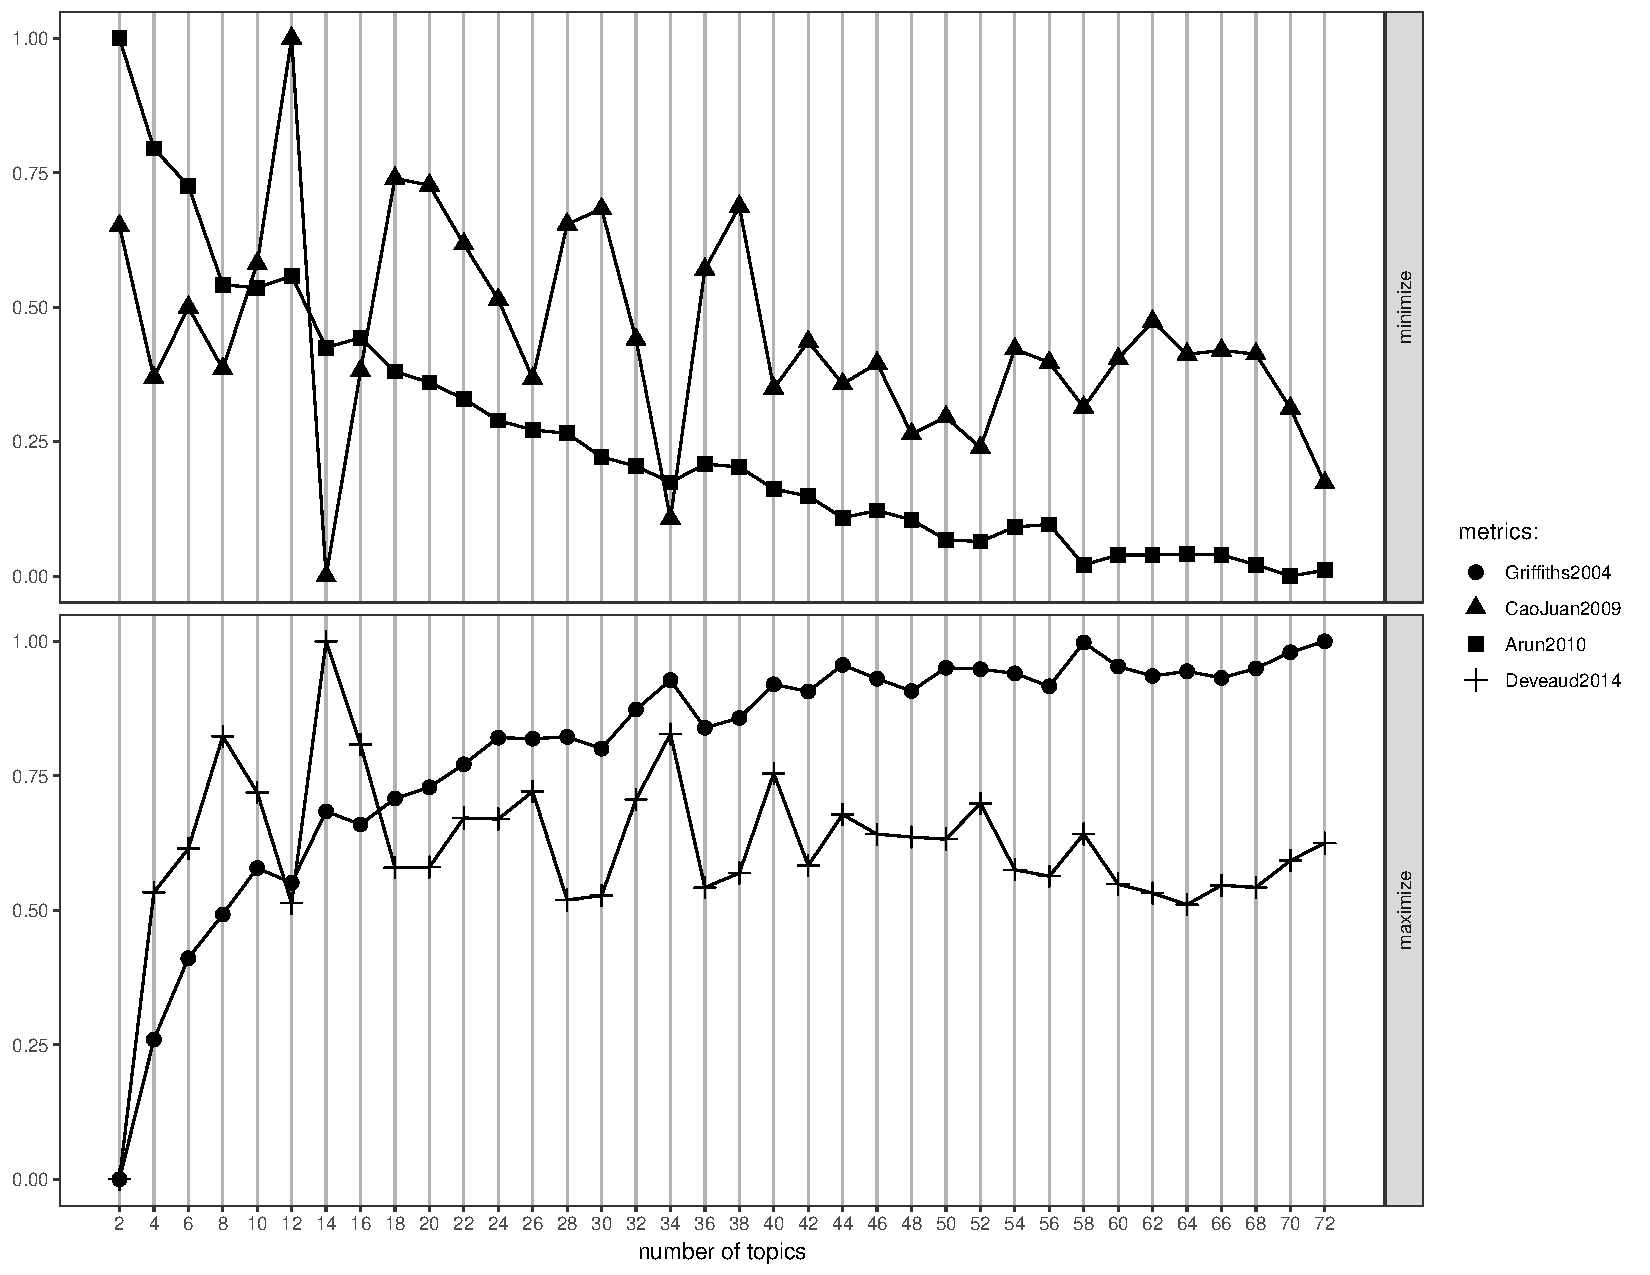
\includegraphics[width=1\linewidth]{Figures/ChapterV/TopicSelection}
	\caption[LDAtuning Ensemble for Determining the Number of Topics in LDA]{LDAtuning ensemble for determining the number of topics in LDA.   As can be seen from the short distance between Deveaud (2014) and CaoJuan (2009) around 14 topics and the close agreement between the Griffiths (2004) and Arun (2010) measure as the number of topics increases - especially after 58.  This suggests that a number of topics should be between 14 and 58.  Within  this band, all 4 metrics are in closest agreement at 34 topics, therefore 34 topics will be used in the LDA analysis.    }
	\label{fig:topicselection}
\end{figure}

\section{Applying the Model to the Data}

After the model is trained, the LDA provides two tables: beta table and gamma table. The first table, beta table, gives the probability of each stock belonging to each topic, whereas the second table, gamma table, contains the probability of each investor belonging to each topic. 


%per-document-per-topic probabilities
\subsection{Per-Topic Probabilities}

Figures \ref{fig:lda34-1-9} to \ref{fig:lda34-28-34} display the 10 stocks with the highest probability of being assigned to each topic.  It should be noted that the order of each topic number is purely arbitrary, and nothing should be read in the rank-order of the different topics, nor the relative distance between topic numbers \citep{Silge2018}.  

Within these topics, some are easier to label than others.  For example, topic 7 appears to be concentrated in Canadian banks as well as energy companies, topic 9 suggests to be a smorgasbord of various ETF and indexed securities, whereas topic 25 appears to be a strong collection of bluechip staples.  

On the other hand, this 34 topic LDA gives us topics that would appear superficially similar, but are treated as different topics.  For example, topics 10 and 13 are anchored by Berkshire Hathaway stock, but the main difference between the two is that topic 13 puts a much larger importance on the acumen of Warren Buffet than topic 10's more diversified approach.  

\begin{figure}
	\centering
	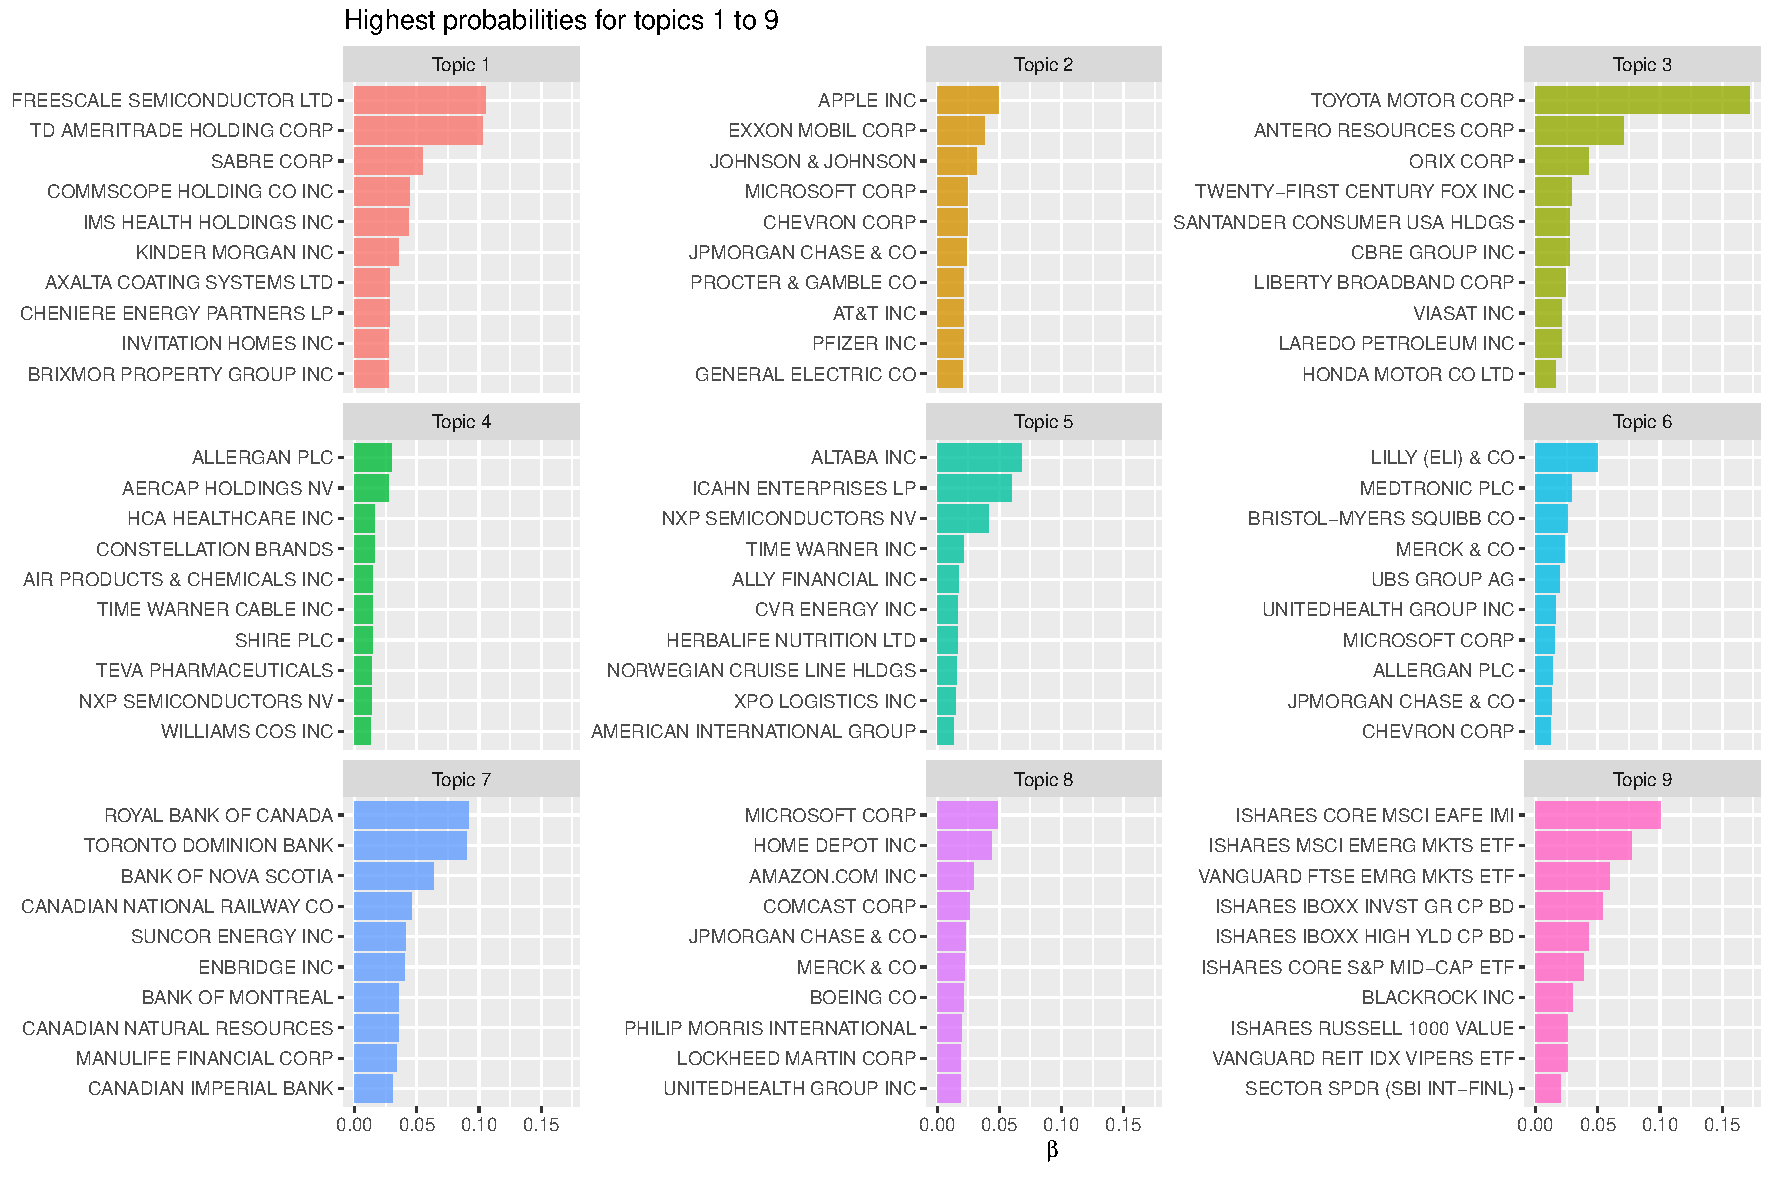
\includegraphics[width=\linewidth]{Figures/ChapterV/LDA34_1-9}
	\caption[Topic Model with 34 Topics, Topics 1 thought 9]{Topic model with 34 topics, topics 1 thought 9. This represents the 10 most likely stocks being associated to a particular portfolio archetype.}
	\label{fig:lda34-1-9}
\end{figure}

\begin{figure}
	\centering
	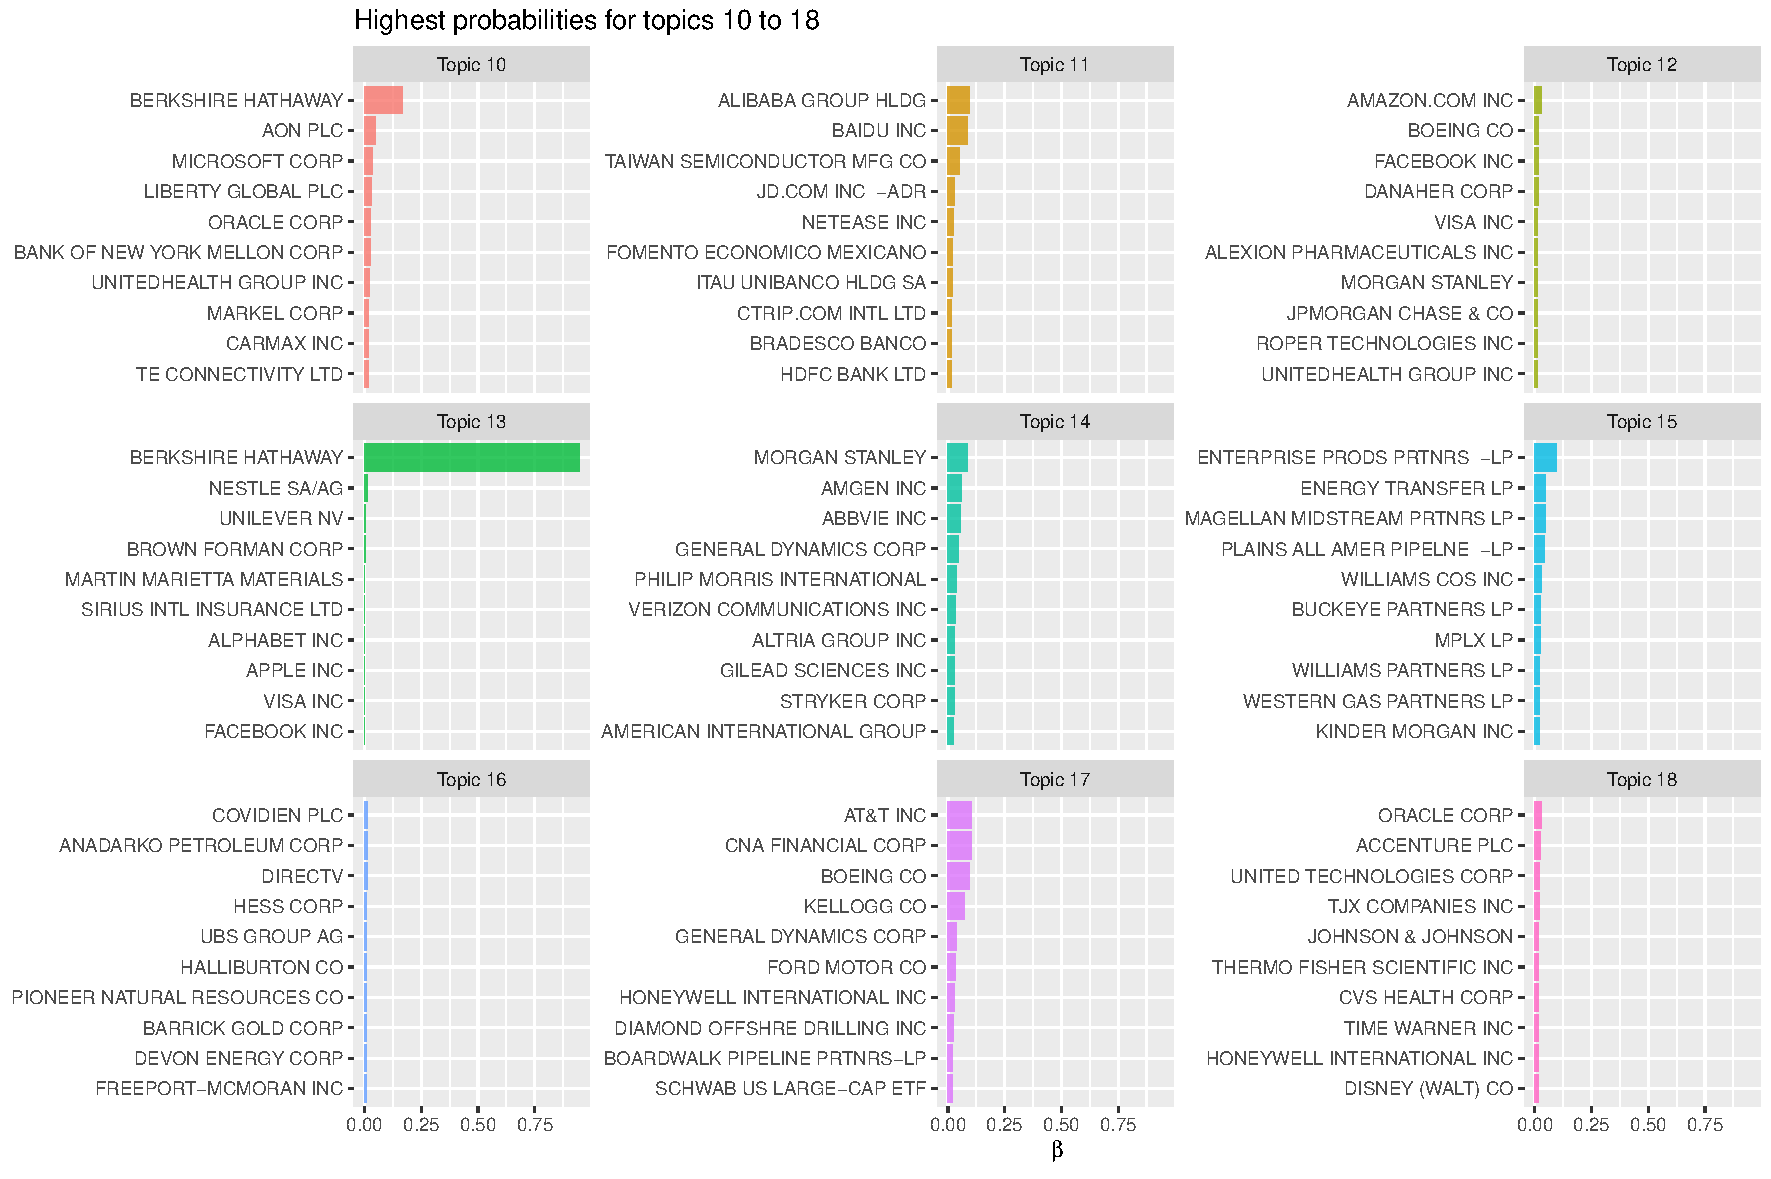
\includegraphics[width=\linewidth]{Figures/ChapterV/LDA34_10_18}
	\caption[Topic Model with 34 Topics, Topics 10 thought 19]{Topic model with 34 topics, topics 10 thought 19. This represents the 10 most likely stocks being associated to a particular portfolio archetype.}
	\label{fig:lda34-10-18}
\end{figure}

\begin{figure}
	\centering
	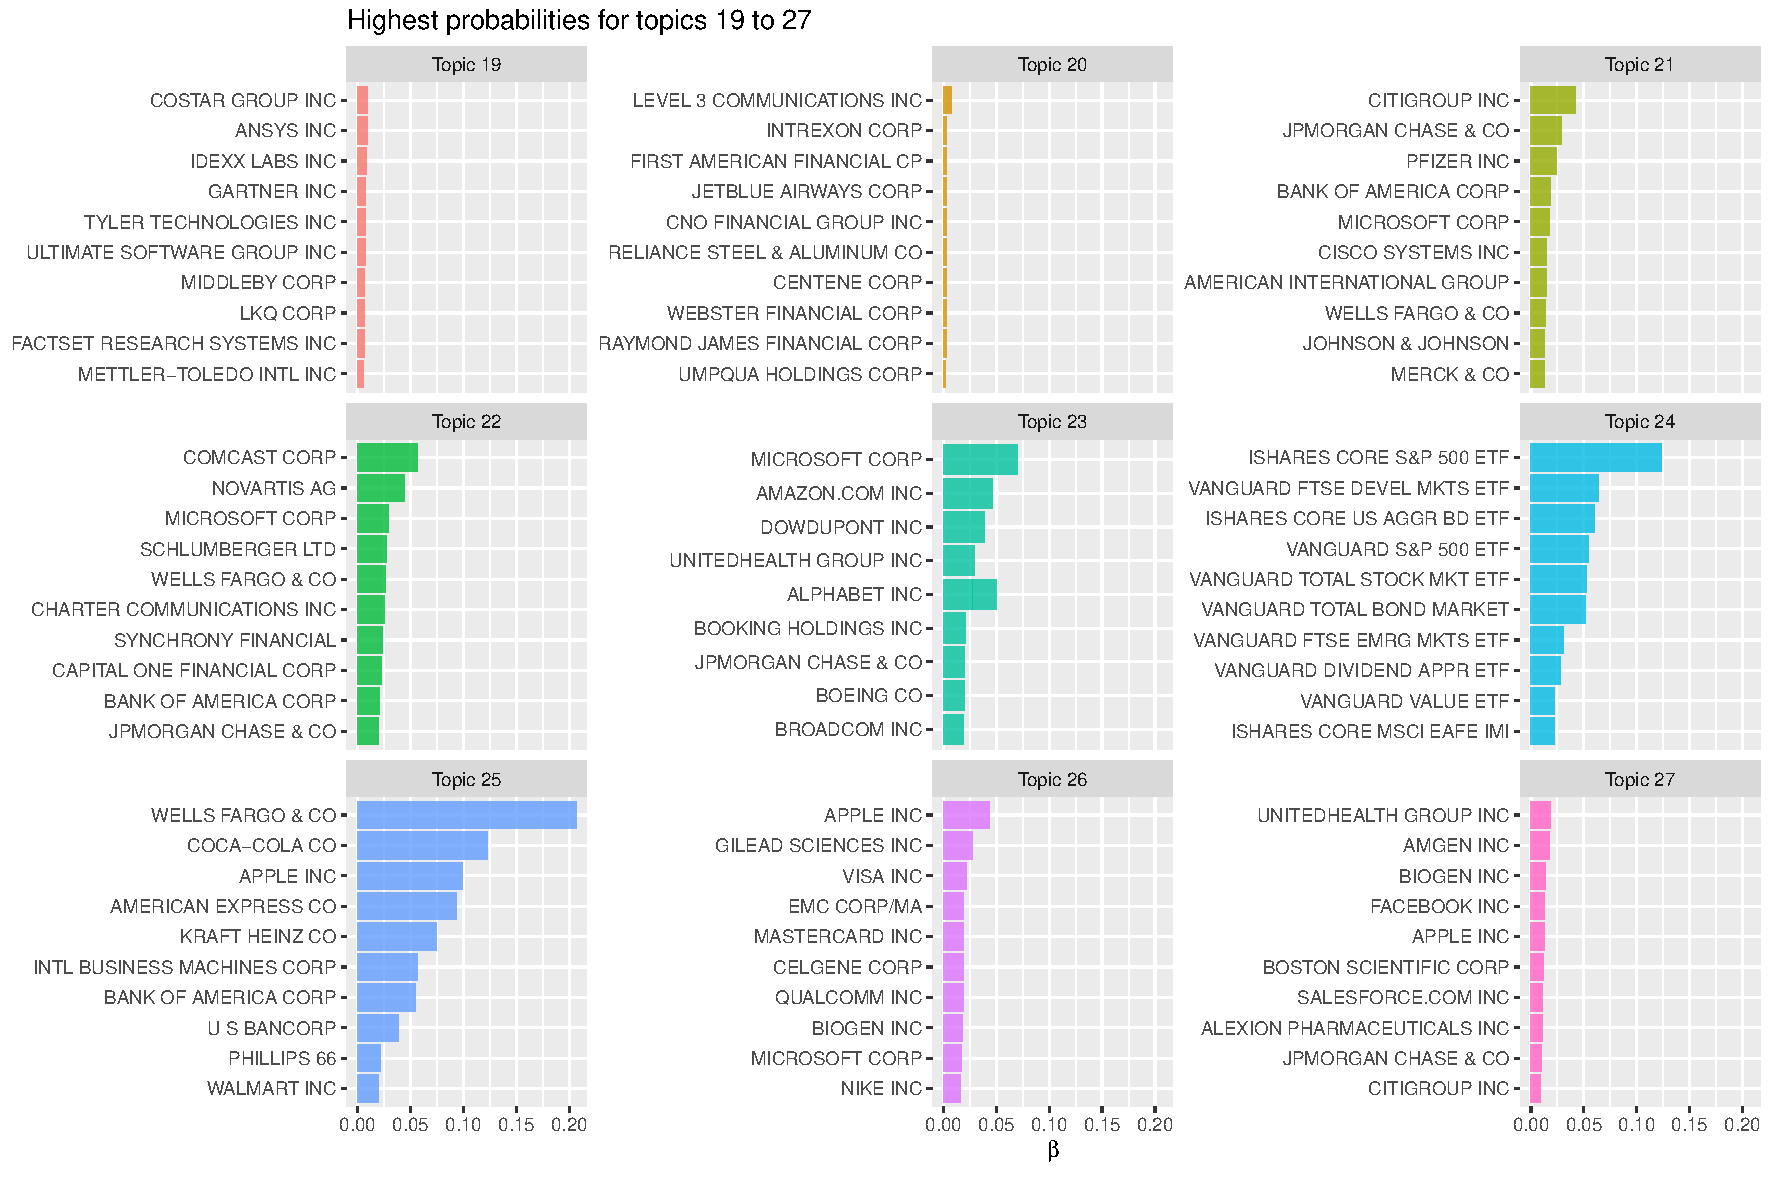
\includegraphics[width=\linewidth]{Figures/ChapterV/LDA34_19_27}
	\caption[Topic Model with 34 Topics, Topics 19 thought 27]{Topic model with 34 topics, topics 19 thought 27. This represents the 10 most likely stocks being associated to a particular portfolio archetype.}
	\label{fig:lda34-19-27}
\end{figure}

\begin{figure}
	\centering
	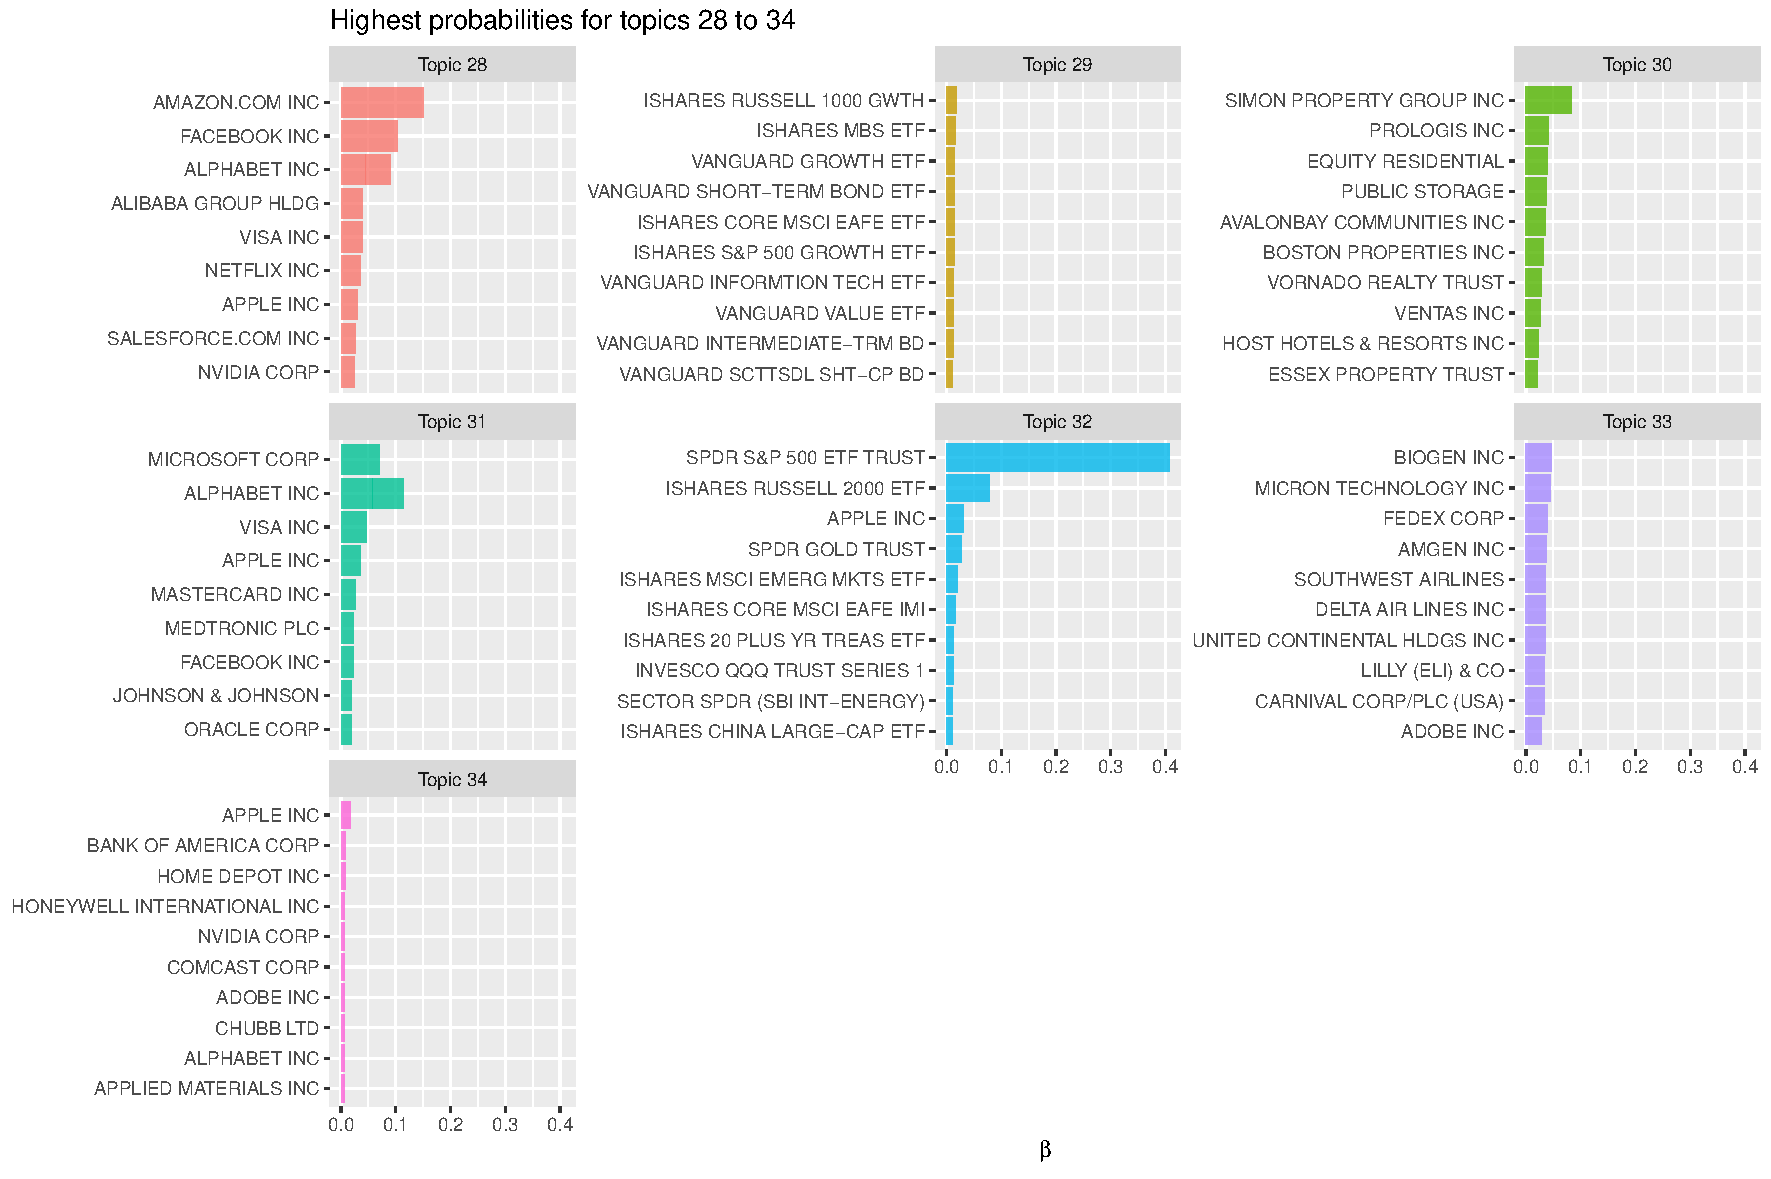
\includegraphics[width=\linewidth]{Figures/ChapterV/LDA34_28_34}
	\caption[Topic Model with 34 Topics, Topics 28 thought 34]{Topic model with 34 topics, topics 28 thought 34. This represents the 10 most likely stocks being associated to a particular portfolio archetype.}
	\label{fig:lda34-28-34}
\end{figure}


\subsection{Per-Document-Per-Topic Probabilities}

The per-document-per-topic probabilities are found in gamma table of the output.  This table aggregates each stock's probability of belonging to a topic for each investor and thus gives the probability of each investor of belonging to each topic.  The aggregate probability of each topic is displayed in Tables \ref{tab:Topics_investors_2013-2014} to \ref{tab:Topics_investors_2017-2018}, giving us an idea of how the popularity of each topic fares over time.  For example, topic 26 saw a precipitous decline from 172.40 to 14.15 aggregate investor probability of belonging to this topic, conversely topic 23 grew from 3.58 to 198.21 in this same metric.  

Given that the investors were already geocoded in a previous chapter, the investors' topic probability was aggregated by State, and Figures \ref{fig:StateLDA1} to \ref{fig:StateLDA34} were created using the geofacet package in R. These geofacet maps allows for the thematic representation of line graphs in a geometric patters that resembles the adjacency of US States, facilitating an easier to grok representation of the data than a series of choropleth maps representing different time slices.  

Looking deeply at the aggregate investor probability tables offer hints at why  certain seemingly related topics, such as topics 10 and 13 -- high concentrations of ETFs -- as mentioned earlier might have a high thematic similarity, however these investors are given high probability classification to one topic and have a correspondingly low probability classification for the other topic.  Going back to the fundamentals of Modern Portfolio Theory (MPT) might give insights into this outcome, and we are simply seeing two broadly similar strategies that are conceptually similar, but use different securities in the process.  Furthermore, a look at the tables \ref{tab:Topics_investors_2013-2014} to \ref{tab:Topics_investors_2017-2018} indicates that these topics are getting more followers over time, however figures \ref{fig:StateLDA10} and \ref{fig:StateLDA13} show that this growth is geographically uneven, given that topic 13 has most of its growth coming from investors located outside of New York State than is the case with topic 10. 

In a more general sense, the maps from Figure \ref{fig:StateLDA1} to \ref{fig:StateLDA34} are a reflection of the national locational trends seen in Chapter \ref{ChapterIII} (Exploring the Data), in that institutional investor firms prefer to locate in places where there are already other institutional investors (mainly NY and to some extent California, Massachusetts and Texas).  Furthermore, this fractional accounting of investment firms by percentage probability of belonging to an investment strategy will reflect this reality.  That being said, this isn't really surprising in light of the literature on location decisions.  \cite{covalthe2001} show that it was the smaller investors that had out-sized returns from pursuing locality-based investment strategies, and that these strategies -- due to the required personal interaction -- would be very hard to scale up.  Secondly, the reliance of HQ location for tying an investor to their location does not preclude an investor having an oil specialist in Houston or Calgary for their oil portfolio research. 

Overall, what does this mean?  Best practices and strategies tend to homogenize portfolios.  Some strategies might be geographically concentrated to a certain extent, but the nature of trading as it is currently practiced has reduced the friction of information transfer, and thus while not quite unshackling the geography of trading, has added additional links to the chains. 

\section{Shift-Share}

Shift-share is a technique used in econometrics and regional studies developed by Edgar Dunn Jr. to ascribe changes in the share of a particular sector of the local economy into 3 main factors: a national factor - how well the global economy is doing; an industry factor - how well a particular industry is doing relative to the global economy; and a regional factor - how well the region is doing taking into account the national and industry trends \citep{dunn1960statistical}.   This last factor is important, since it allows various regions to see how they are doing relative to the set of global and industry headwinds.  Similarly, the use of regional shifts to measure how well a region is doing with regards to an investment topic is useful for determining the health a given strategy  when keeping with the investment topic as a whole and the national trends. 

The equation for shift share is as follows:
\begin{equation}
   e^{t+n}_{i} - e^{t}_{i} = NS_{i} + IM_{i} + RS_{i}
    \label{Eq:Shft_share}
\end{equation}

Where $e$ is the shift-share in industry $i$ between the time periods $t$ and $t+n$.  This shift-share is the sum of the three effects: national growth effect ($NS_{i}$), the industry mix effect ($IM_{i}$) and the local shift ($RS_{i}$). 

The national share is calculated as follows:

\begin{equation}
    NS = e^{r}_{i}g^{n}
    \label{Eq:NationalShare}
\end{equation}

The industry mix is calculated as follows:
\begin{equation}
    IM = e^{r}_{i}(g^{n}_{i} - g^{n})
    \label{Eq:IndustryMix}
\end{equation}
and the regional shift is calculated as follows: 
\begin{equation}
    RS =  e^{r}_{i}(g^{r}_{i} - g^{n}_{i})
    \label{Eq:RegionalShare}
\end{equation}

Where $e^{r}_{i}$ is the value in Sector $i$ in Region $r$ at the beginning of the period, $g^{n}$ is the growth rate for the value for the total area under study over the time period, $g^{n}_{i}$ is the growth rate of Sector $i$ for the total area under study for the time period, and $g^{r}_{i}$ growth rate in sector $i$ in Region $r$ for the time period \citep{Houston67}. 

\subsection{Dynamic Shift-Share}

However, as the release of data became more granular, both in terms of time period and geography, a more nuanced version of shift-share was developed: the dynamic shift-share.  This version of shift-share takes into account the period to period fluctuations by performing the shift-share in a time-series and adding together all of the shifts \citep{BarffKnight88}.  Since this model uses a time-series, it is less vulnerable to effects caused by choosing the start and end years. Furthermore, \cite{BarffKnight88} as well as \cite{harris1994dynamic} show that the use of a dynamic shift-share with regular reporting periods (as is the case of 13F-HR data) means that there is less of a compounding effect. That is to say that one abnormally large change in a short period of time in the data creates a change in regional-shift that is disproportional to the underlying trend. In this case, this could be exemplified by the start-up of one large fund entering the data-set and having a profound quarter-to-quarter change in the data during the quarter it entered and then returning to a national growth rate.  The dynamic shift-share is better prepared to deal with this type of data intrusion.  

The dynamic shift-share is written as follows:

\begin{equation}
    e^{t+n}_{i} - e^{t}_{i} = NS_{i} + IM_{i} + RS_{i}
\end{equation}

If the study period ranges from year $t$ to year $t+n$, the traditional shift-share effects are calculated for every year $k$, where k spans from $t+1$ to $t+n$. 

\begin{equation}
    NS_{i} = \sum_{k=t+1}^{t+n}[e^{k-1}_{i}(G^{k})]
    \label{Eq:NationalShare_dynamic}
\end{equation}

\begin{equation}
    IM_{i} = \sum_{k=t+1}^{t+n}[e^{k-1}_i(G^{k}_{i}-G^{k})]
     \label{Eq:IndustryMix_dynamic}
\end{equation}

\begin{equation}
    RS_{i} = \sum_{k=t+1}^{t+n}[e^{k-1}_i(g^{k}_{i} - G^{k}_{i} )]
        \label{Eq:RegionalShare_dynamic}
\end{equation}

For the dynamic model shift-share, Equation \ref{Eq:NationalShare_dynamic} replaces Equation \ref{Eq:NationalShare} for the national share, Equation \ref{Eq:IndustryMix_dynamic} replaces Equation \ref{Eq:IndustryMix}  for the industry mix and Equation \ref{Eq:RegionalShare_dynamic} replaces Equation \ref{Eq:RegionalShare} for the regional share.  The dynamic model shift-share is then calculated at the sum of the annual effects \citep{BarffKnight88}.  

In this case, rather than calculate yearly effects for $k$, this application of the dynamic shift-share used each quarterly filing between the second quarter of 2013 to the fourth quarter of 2018, therefore creating 23 discreet time steps.

The analysis was performed using \cite{Soudis2019} R package implementation for dynamic shift-share. The holdings of each portfolio was weighted by the $\beta$ of each topic/portfolio archetype as determined by the 34 topic LDA analysis, and summed by relevant geography. The results in tabular form are in Appendix \ref{appendix:shiftshare}.

By taking the regional shift values and then mapping them onto a map of the USA, this displays the local/regional effects of a given topic/portfolio archetype in a given geography while keeping the overall growth of the stock market and the varying popularity of a particular strategy constant. In order to minimize the role of outlier-values over-exposing the linear scale of the regional-shift, the regional shifts were binned into 10 categories using the Jenks method via the ClassInt package in R \citep{classInt}.  The Jenks natural-breaks method classifies continuous data by grouping them iteratively into $k$ groups such that it maximizes the square of variance between groups and minimizes the square of variance within groups \citep{jenks1967data}.  


\section{Regional Results}

Throughout the ensemble of the 34 maps displaying the regional shifts for the continental USA, a re-occurring theme is that New York State and the State of California are often at odds with one-another. In the majority of these cases, New York State has a positive regional-shift value, and California has a corresponding negative shift value, whereas the reverse is only true in two cases: topic 13 (majority Berkshire Hathaway) and topic 32 (mostly broad sector and indexed ETFs).   The question then becomes, why is California suffering such as persistent subordinate position to New York despite being ranked second in the number of firms and firm growth during the time period of 1999 to 2018?  

Assuming a scenario in which New York State isn't at the centre of the US financial system would strain the credulity of the credulous considering that Wall Street has been the byword of the US financial and business concerns for nearly a hundred years.  New York is not only number 1 in terms of absolute number of new firms, but also these firms proportionally handle more money (see Chapter \ref{ChapterIII}).  While California's tech sector might be a massive economic engine, these investment firms growing in San Francisco and Los Angeles are smaller than the new firms in New York City and Manhattan in particular. This may be explained by leaning into New York City's historic role as the United States' financial centre as well as California's history as a centre of venture capital driven investment.  

First of all, the preeminent position of Wall Street and the Financial District is further cemented by the wave of consolidation in the aftermath of the Great Financial Crisis of 2008 \citep{wheelock2011banking}. In fact, New York is home to 5 of the 8 systemically important banks located in the USA\footnote{Morgan Stanley, JPMorgan Chase, Goldman Sachs, Citigroup and Bank of NY Mellon}, and 2 of the 3 other banks have substantial operations in New York\footnote{Wells Fargo has its official Headquarters in San Francisco and a substantial operation in the Seagram Building on Park Avenue,  Bank of America has substantial operations in New York in the Bank of America Tower on Sixth Avenue}, while the remaining is State Street headquartered out of Boston Massachusetts \citep{FSB2019}. 


As to why California lags behind may well be an artifact of the dataset, for California is quite famous for its venture capital investment culture \citep{greenventure2004} and its large herd of unicorns\footnote{A unicorn is a private start-up with a valuation above one billion USD. \citep{Lee2013}} \citep{kenney2019unicorns}. This long history of venture capital-backed firm creation model gives an enticing hint that there is a substantial pool of money in California that exists largely outside of the 13F-HR universe, since privately held corporations as well as stocks for firms that are not publicly listed do not show up in 13F-HR reports.  Furthermore, due to recent changes in American regulations for start-ups, 2012's JOBs Act in particular allowing for greater number of qualified investors in a company before requiring companies to go public, has incentivized institutional capital to invest in star-ups prior to their initial public offering (IPO), as well as delaying the need for firms to create an IPO in order to access the capital needed to grow their company \citep{kenney2019unicorns}.

\nomenclature{IPO}{Initial Public Offering}

As per \cite{florida2016rise}, California contains four of the top 6 metro areas for venture capital, with the San Francisco Bay area (San Francisco and San Jose) accounting for nearly one of every four dollars invested in venture capital nationwide, and Southern California (Los Angeles, San Diego and Orange County) when taken collectively outranks New York City. Furthermore, \cite{adams2018diversified} shows that the investment culture of the San Francisco Bay area prioritized plowing back the capital gained from previous ventures such as gold mining, shipping and the military-industrial complex into new ventures directly rather than invest in the stock market. 

In their most recent report  the National Venture Capital Association\citeyearpar{NVCA2020} -- a national trade and lobbying organization for venture capital firms -- found that for the  years of this study (2013 to 2018), the total funds under management for venture capital firms headquartered in California grew from 128.7 billion to 241.9 billion USD (annual average growth of 22.24 billion USD), whereas in the same time period, New York grew from 26.9 billion to 56.3 billion (annual average growth of 4.925 billion USD). While the  National Venture Capital Association data shows a strong growth trend for venture capital investing for VC firms located in California, it should be re-iterated that capital will flow like water towards where it anticipates future returns.  As such, there is no mechanism preventing a VC fund in California from investing in a NY based start-up, and similarly, there is no mechanism preventing a NY based institutional investor from investing in a Silicone Valley tech giant. That being said, the report notes that there is a strong local bias in venture capital investment patterns. 


\nocite{NVCA2020data}



\begin{figure}
	\centering
	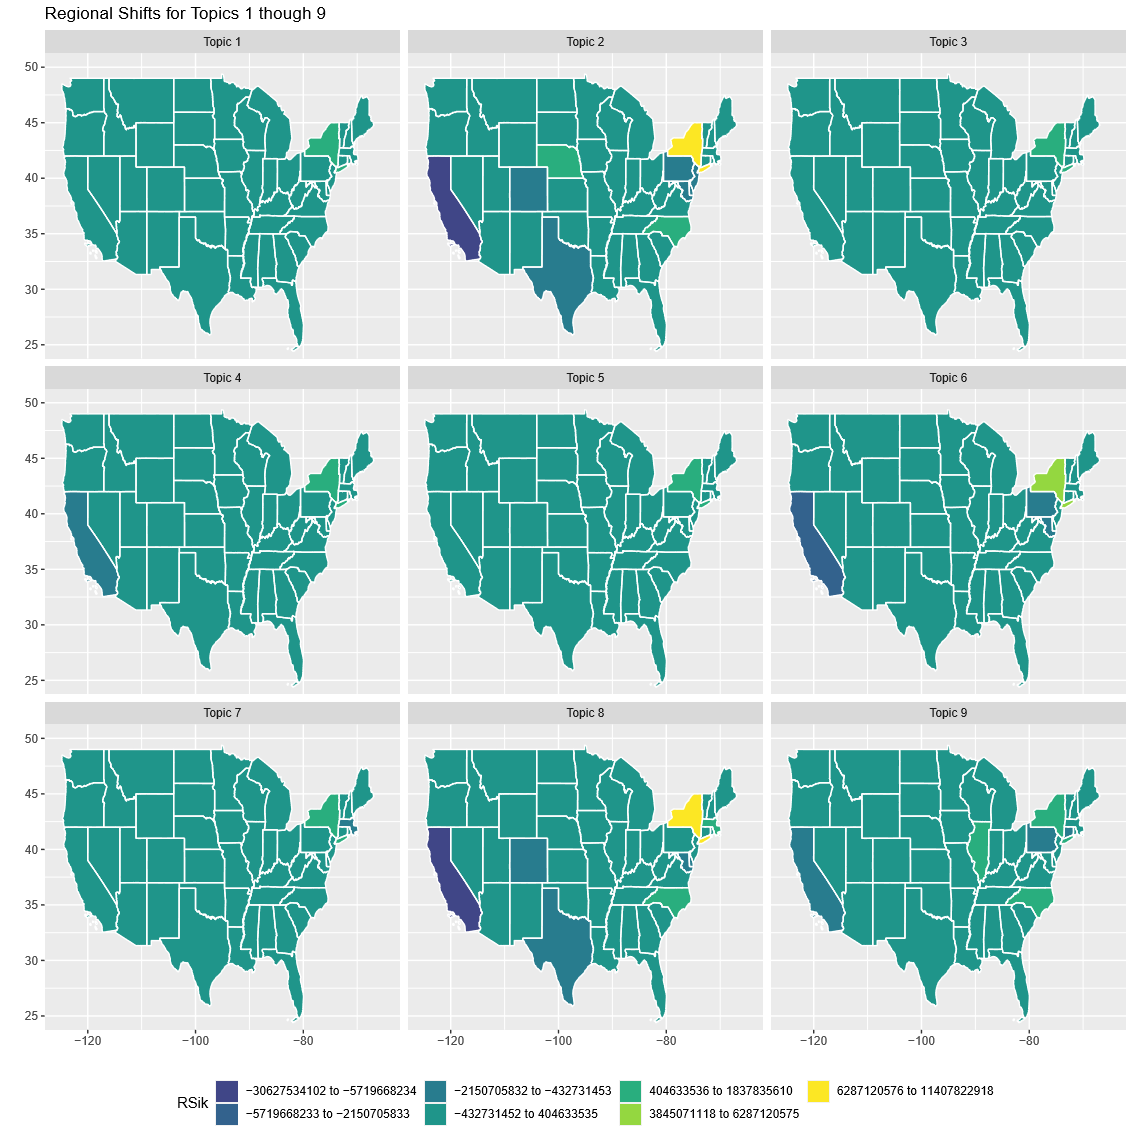
\includegraphics[width=\linewidth]{Figures/ChapterV/States_01_09}
	\caption[Regional Shifts using 34 Topic LDA, Topics 1 thought 9]{Regional shifts for topics 1 though 9 of the 34 topic LDA for the Continental USA.}
	\label{fig:shift-share_lda34-1-9}
\end{figure}

\begin{figure}
	\centering
	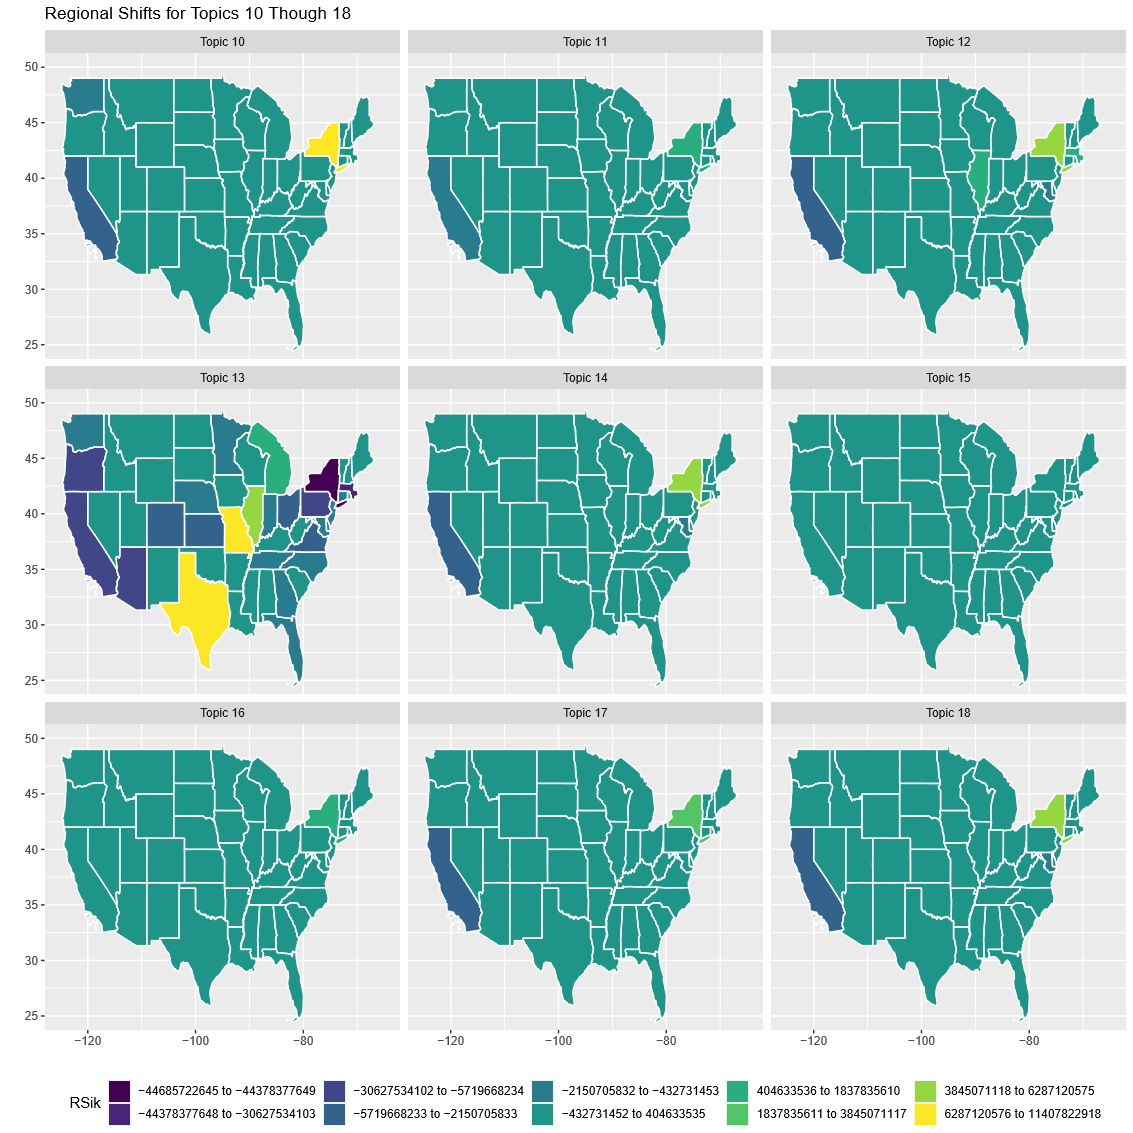
\includegraphics[width=\linewidth]{Figures/ChapterV/States_10_18}
	\caption[Regional Shifts using 34 Topic LDA, Topics 10 thought 19]{Regional shifts for topics 10 though 18 of the 34 topic LDA for the Continental USA.}
	\label{fig:shift-share_lda34-10-18}
\end{figure}

\begin{figure}
	\centering
	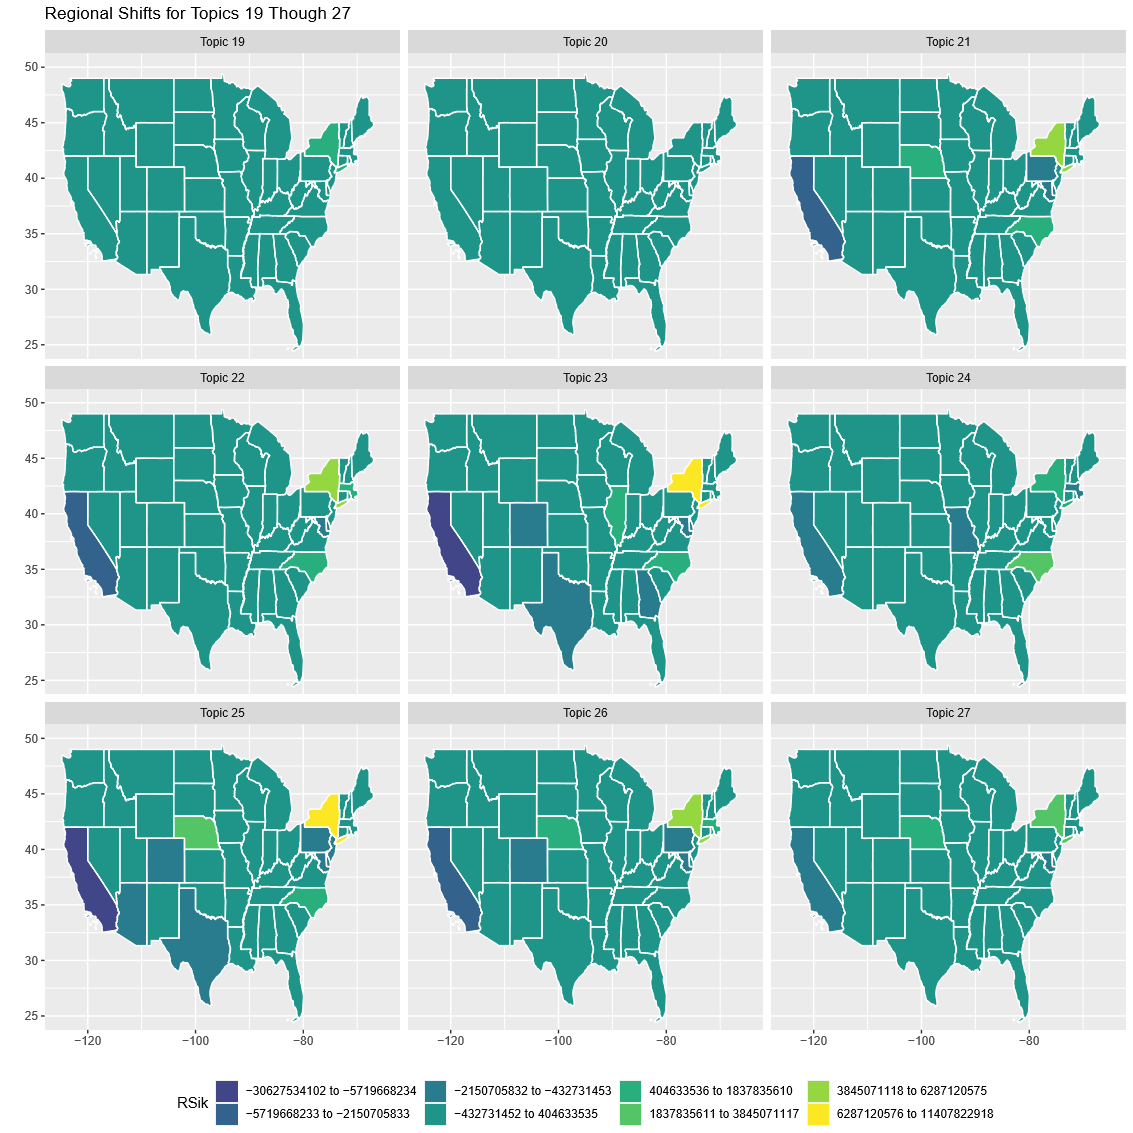
\includegraphics[width=\linewidth]{Figures/ChapterV/States_19_27}
	\caption[Regional Shifts using 34 Topic LDA, Topics 19 thought 27]{Regional shifts for topics 19 though 27 of the 34 topic LDA for the Continental USA.}
	\label{fig:shift-share_lda34-19-27}
\end{figure}

\begin{figure}
	\centering
	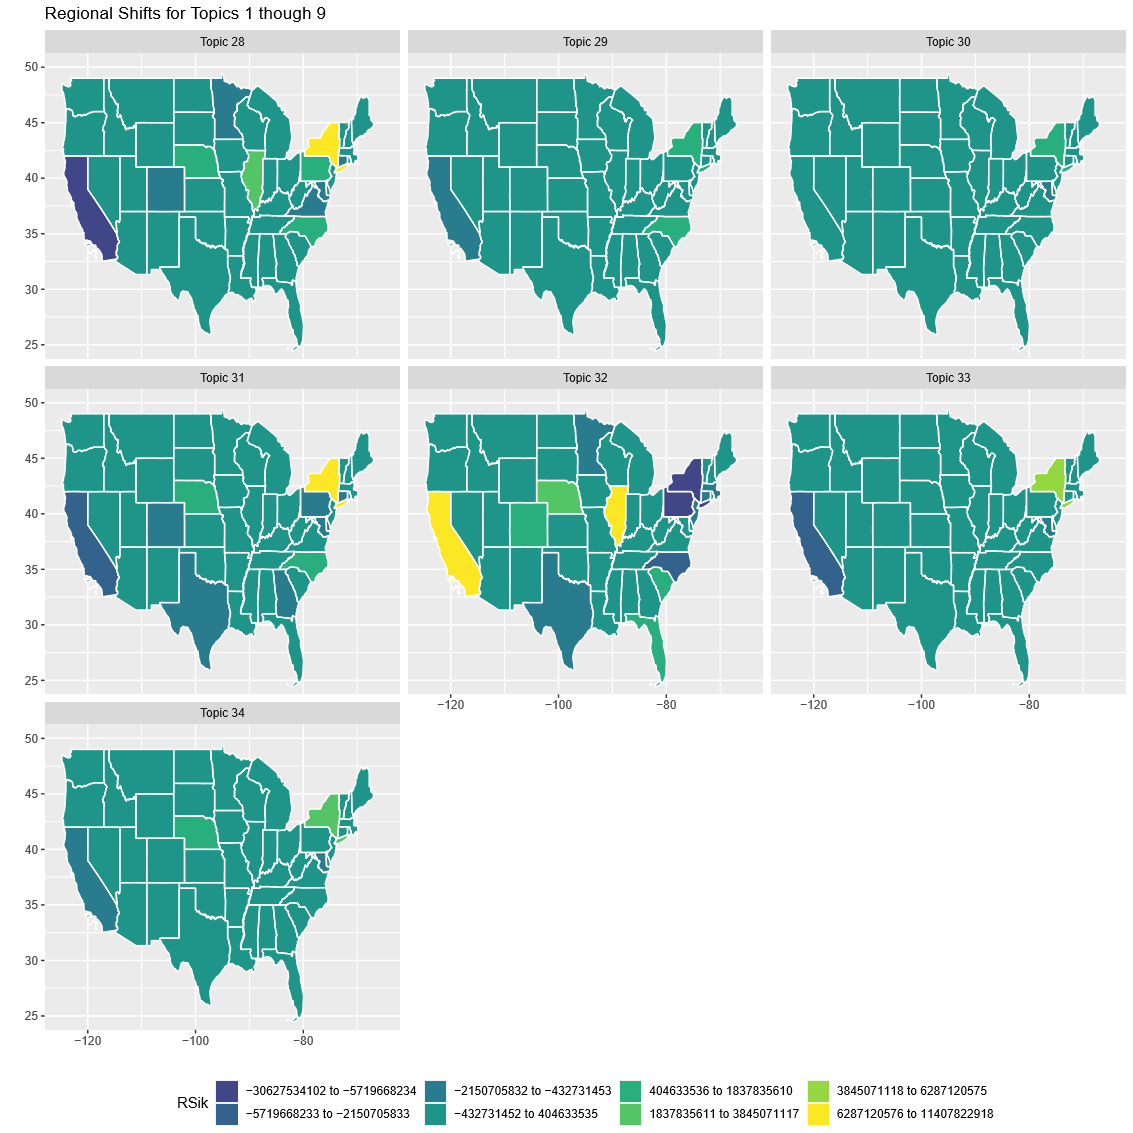
\includegraphics[width=\linewidth]{Figures/ChapterV/States_28_34}
	\caption[Regional Shifts using 34 Topic LDA, Topics 28 thought 34]{Regional shifts for topics 28 though 34 of the 34 topic LDA for the Continental USA.}
	\label{fig:shift-share_lda34-28-34}
\end{figure}

\begin{figure}
    \centering
	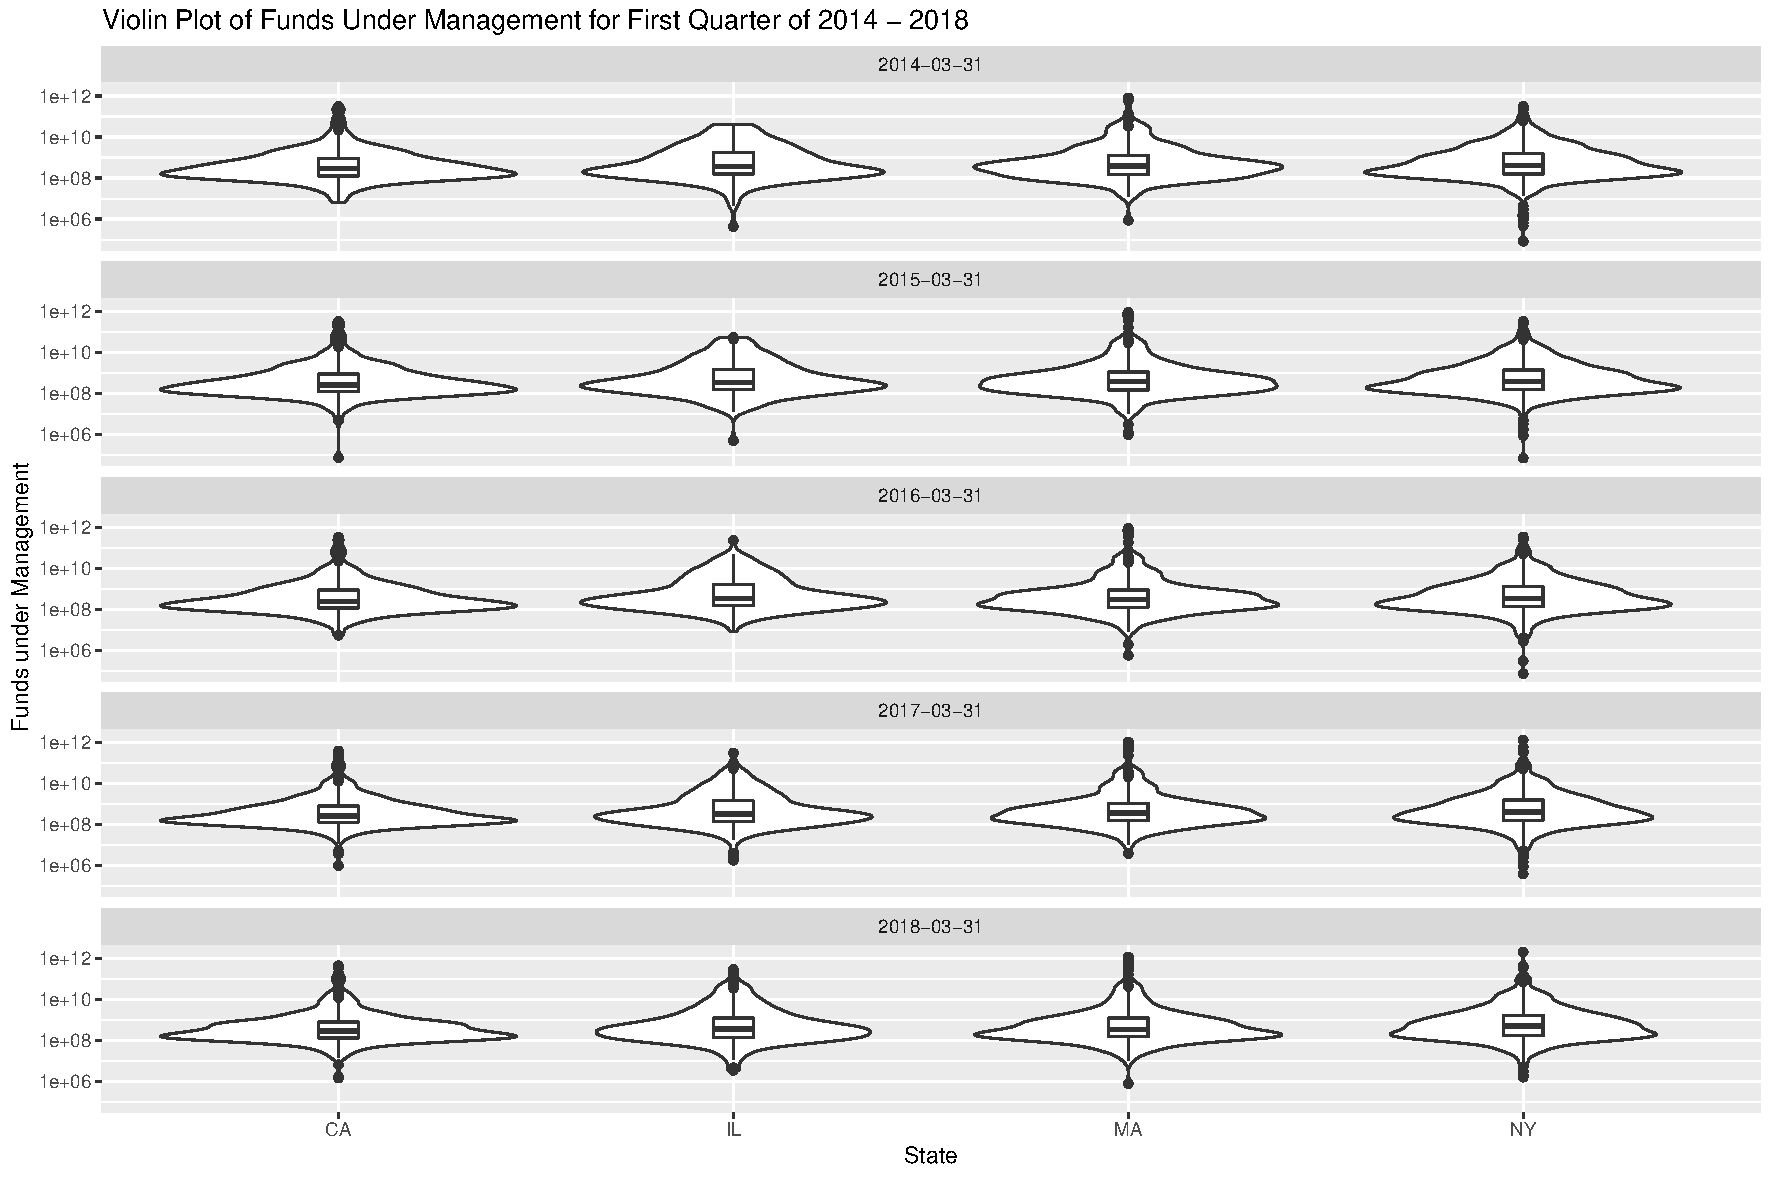
\includegraphics[width=1\linewidth]{Figures/ChapterV/Violinplot_q1}
	\caption[Violin Plot of Firm Holding Size for CA, IL, MA and NY.]{Violin plot of firm holding size for the States of California, Illinois, Massachusetts and New York.}
	\label{fig:violinplotq1}
\end{figure}


In light of this marked difference between New York and California, the absence of the number 2 and three 3 cities in the rank-order of metro areas by funds under management, Boston and Chicago are the dogs that didn't bark\footnote{In Arthur Conan Doyle's "Silver Blaze", the absence of barking from the guard dogs narrowed down the list of suspects since they had to be known to the dogs -- hence the lack of barking at an intruder -- and allowed Sherlock Holmes to crack the case.}.  In this case, Boston and Chicago have firm size distribution that is similar to New York and California (Figure \ref{fig:violinplotq1}), however these two large second tier cities drive the middle road between California's penchant for VC investment and New York's role as a stock-trading  nexus.

\section{Conclusion}

Overall, the LDA analysis did not show much geographical segregation.  This is to be somewhat expected given the homogenization of investment best-practices, and the long shadow of the Efficient Market Hypothesis.  That being said, the shift-share analysis on the resulting LDA topics underscores the massive difference in stock investing funds under management growth over time between New York and California. While not obvious in term of top line numbers for funds under management, number of firms, and the distribution of size of firms by funds under management, this LDA analysis and shift-share show a massive difference between New York and California. Furthermore, while the democratization of institutional investor locations in the USA made it possible to run an institutional investor firm outside of New York City, New York State's very strong growth for funds under management across the multitude of different investment strategies belies New York City's strength as a financial nexus.  Or put another way, California's weakness in the institutional investor game is akin to the odd perturbations of Jupiter and Saturn's orbits that could not be explained until the discovery of Uranus and Neptune during the later half of the 19\textsuperscript{th} century.  

